\chapter{Problem Definition and Algorithms}

In this chapter we will formally define the query optimization problem in the
context of temporal relational databases.

\section{Problem definition}
Keeping the historical records of transactions on a database system is useful because it stores the entire updates of a database. In our proposed system these historical records could be used to regenerate the form of a table (snapshot) or a record in a specific timestamp. Also, cryptographic techniques could be used to create a cryptographic chain in order to secure these records from tampering, therefore by investigating the authenticity of all transactions applied to an specific record throughout its lifecycle, the trustworthiness of that record could be ensured. Append-only temporal relational tables, if chosen for keeping the historical records, are beneficial because not only they are simple to implement, but also there is the luxary of having RDBMS to manage and perform queries on such tables.

\textbf{Example.} Definition of a timeline was introduced in \textbf{Definition 4}. The historical records obtained from auditing the database transaction could be seen as a timeline. A request to regenerate the form of a table (snapshot) or a record can be depicted in \ref{fig:snapshot_notion}

\begin{figure}
	\label{fig:snapshot_notion}
	\centering
	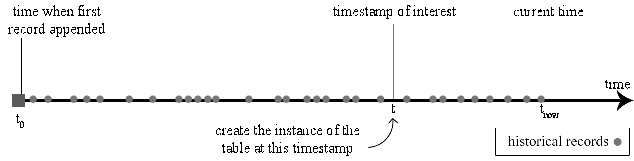
\includegraphics[width=\textwidth]{figs/snapshot_notion.pdf}
	\caption{The notion of creating snapshot on the timeline.}
\end{figure}


\textbf{Proposition. Linear time in creating snapshots}:The notion of creating a snapshot which shows the instance of the table $r$ in a certain timestamp $t$, using historical records stored in an append-only temporal relational table $r^T$ defined in \textbf{Definition 5}. Assume that the tables are updated at a constant rate over time, then the complexity of $\mathrm{snapshot}(r, t)$ is $$\mathcal{O}(|\{x: x\in r^T\mathrm{\ and\ } x.\mathrm{updates} \leq t\}|)\simeq \mathcal{O}(t)$$
Since $r^T$ could be seen as a timeline, the records which needs to be checked can be depicted in \ref{fig:checked_records}. This clearly indicates that a linear time is required to compute a snapshot at a timestamp of interest and as the size of $r^T$ grows in size, creating snapshot become computationally more expensive.

\begin{figure}[b]
	\label{fig:checked_records}
	\centering
	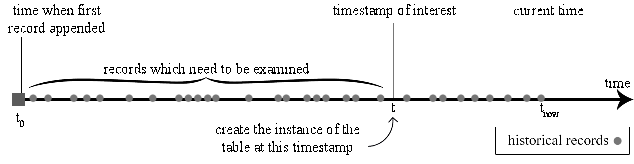
\includegraphics[width=\textwidth]{figs/tobechecked_records.pdf}
	\caption{The records which needs to be checked when creating a snapshot.}
\end{figure}

\textbf{Example.} Given a normal relational table $r_1$ (Table \ref{table:normal_table_2}) and a temporal relational table $r_1^T$ (Table \ref{table:temporal_table_2}) which contains the historical data of $r_1$, the $r_1$ at $t=2018-04-01$ looked like Table $\ref{table:normal_table_2_t}$
\begin{center}

\begin{table}[t]
	\centering
	\caption{Normal Relational Table $r_1$}
	\label{table:normal_table_2}
	\begin{tabular}{p{4cm}p{4cm}p{4cm}}
		\hline
		id & item      & value  \\ \hline
		22 & Pencil    & 7.50 \\
		23 & Notebook & 12.0   \\ 
		24 & Console & 230.0 \\ \hline
	\end{tabular}
\end{table}

\begin{table}[t]
	\centering
	\caption{Temporal Table $r_1^T$}
	\label {table:temporal_table_2}
	\begin{tabular}{p{1cm}p{2cm}p{3cm}p{3cm}p{2cm}}
		\hline
		id & item      & value  & updated  & deleted\\ \hline
		21 & Ruler    & 3.25  & 2018-02-10  &  - \\  
		22 & Pencil    & 8.0  & 2018-03-21  &  - \\
		22 & Pencil    & 9.0  & 2018-03-30  &  -\\
		23 & Notebook & 11.0  & 2018-04-01 & - \\
		22 & Pencil & 6.0  & 2018-04-01 & - \\
		21 & Ruler    & 3.25  & -  &  2018-04-02 \\
		23 & Notebook & 12.0  & 2018-04-02 & - \\ 
		22 & Pencil & 7.50  & 2018-04-05 & - \\ 
		24 & Console & 230.0  & 2018-04-05 & - \\ \hline
	\end{tabular}
\end{table}
\begin{table}
	\centering
	\caption{Normal Relational Table $r_1$ at t = 2018-04-01}
	\label{table:normal_table_2_t}
	\begin{tabular}{p{4cm}p{4cm}p{4cm}}
		\hline
		id & item  & value  \\ \hline
		21 & Ruler & 3.25 \\
		22 & Pencil & 6.0   \\ 
		23 & Notebook & 11.0 \\ \hline
	\end{tabular}
\end{table}
\end{center}

\subsection{Query answering using snapshots} 

Using precomputed materialized view has been proven to be effective \cite{sohrabi2016materialized} \cite{du2017deepsea}. Since running queries $Q(t)$ on temporal table $r^T$ to build snapshots or generate latest version of a record at a timestamp of interest requires linear time, we propose to first precompute $n$ number of snapshots $snapshot_i(r,t)$ for materialization and then evaluate $Q$. If some snapshots are precomputed and materialized, then we can save on computational cost in answering the query $Q(t)$. The notion of having precomputed snapshots for materialization can be depicted as Figure \ref{fig:snapshot_materialization}.

\begin{figure}[t]
	\label{fig:snapshot_materialization}
	\centering
	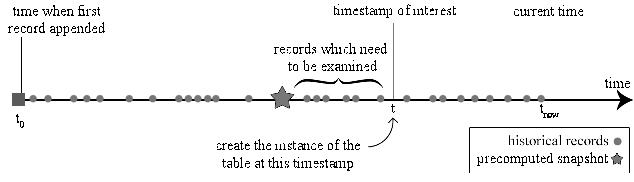
\includegraphics[width=\textwidth]{figs/snapshot_materialization.pdf}
	\caption{The records which needs to be checked when creating a snapshot with having a precomputed snapshot for materialization.}
\end{figure}

\textbf{Proposition} suppose we have a materialized snapshot $snapshot(r,s)$. Then $snapshot(r,t)$ can be computed with complexity:
$$\mathcal{O}(|\{x: x\in r^T\mathrm{\ and\ } x.\mathrm{updates} \in [s,t]\}|) \simeq \mathcal{O}(|s-t|)$$

\textbf{Example.} Given a temporal relational table $r_1^T$ (Table \ref{table:temporal_table_3}) and a precomputed snapshot table $s_1$, we are interested to create the snapshot of table $r_1$ at a timestamp of $t = 2018-03-15$. snapshot $s_1$ is the instance of $r_1$ at $t= 2018-03-11$Table \ref{table:snapshot} shows the records which needs to be evaluated without snapshot materialization and Table \ref{} shows the records which are needed to be evaluated with snapshot materialization.


\begin{center}

\begin{table}
	\centering
	\caption{Temporal Table $r_1^T$}
	\label {table:temporal_table_3}
	\begin{tabular}{p{1cm}p{2cm}p{3cm}p{3cm}p{2cm}}
		\hline
		id & item & value  & updated  & deleted\\ \hline
		1 & Paper & 0.25  & 2018-02-10  &  - \\  
		2 & Scissors & 8.0  & 2018-02-12  &  - \\
		3 & Folder & 1.50  & 2018-02-12  &  - \\
		1 & Paper & 0.30  & 2018-02-13  &  - \\
		4 & Pencil & 3.0  & 2018-02-16  &  - \\
		3 & Folder & 1.75  & 2018-02-21  &  - \\
		5 & Batteries & 8.0  & 2018-02-23  &  - \\
		1 & Paper & 0.35  & 2018-02-25  &  - \\
		6 & Notebook & 7.0  & 2018-03-01  &  - \\
		5 & Batteries & 9.0  & 2018-03-01  &  - \\
		4 & Pencil & 3.25  & 2018-03-04  &  - \\
		1 & Paper & 0.35  &  - &  2018-03-04 \\
		7 & Ruler & 4.0  & 2018-03-06  &  - \\
		2 & Scissors & 8.5  & 2018-03-07  &  - \\
		7 & Ruler & 4.50  & 2018-03-08  &  -\\
		5 & Batteries & 11.0  & 2018-03-10 & - \\
		3 & Folder & 1.75  & - & 2018-03-11 \\
		7 & Ruler & 4.50  & -  &  2018-03-12 \\
		6 & Notebook & 7.50  & 2018-03-15 & - \\ 
		2 & Scissors & 7.50  & 2018-03-17 & - \\ \hline
	\end{tabular}
\end{table}
\begin{table}
	\centering
	\caption{Snapshot of $r_1$ at t = 2018-04-01}
	\label{table:snapshot}
	\begin{tabular}{p{4cm}p{4cm}p{4cm}}
		\hline
		id & item  & value  \\ \hline
		1 & Paper & 0.35 \\
		2 & Scissors & 8.25   \\ 
		4 & Pencil & 3.25   \\ 
		5 & Batteries & 11.0   \\ 
		6 & Notebook & 7.0 \\ 
		7 & Ruler & 4.50   \\ \hline
	\end{tabular}
\end{table}
\end{center}



\section{Optimal single snapshot placement}

\section{A recursive algorithm for optimal snapshot placements}

\section{Dynamic programming approach to optimal snapshot placements}

\section{Heuristic snapshot placements}

\section{Discussion}
